\documentclass{rapport}
\usepackage{lipsum}
\usepackage{tikz}
\usepackage{wrapfig}
\usepackage{caption}
\usepackage{hyperref}
\title{Rapport Visuwalk} %Titre du fichier

\begin{document}

%----------- Informations du rapport ---------

\unif{EURECOM}
\titre{S5 PROJECT REPORT :\\ 
\begin{center}
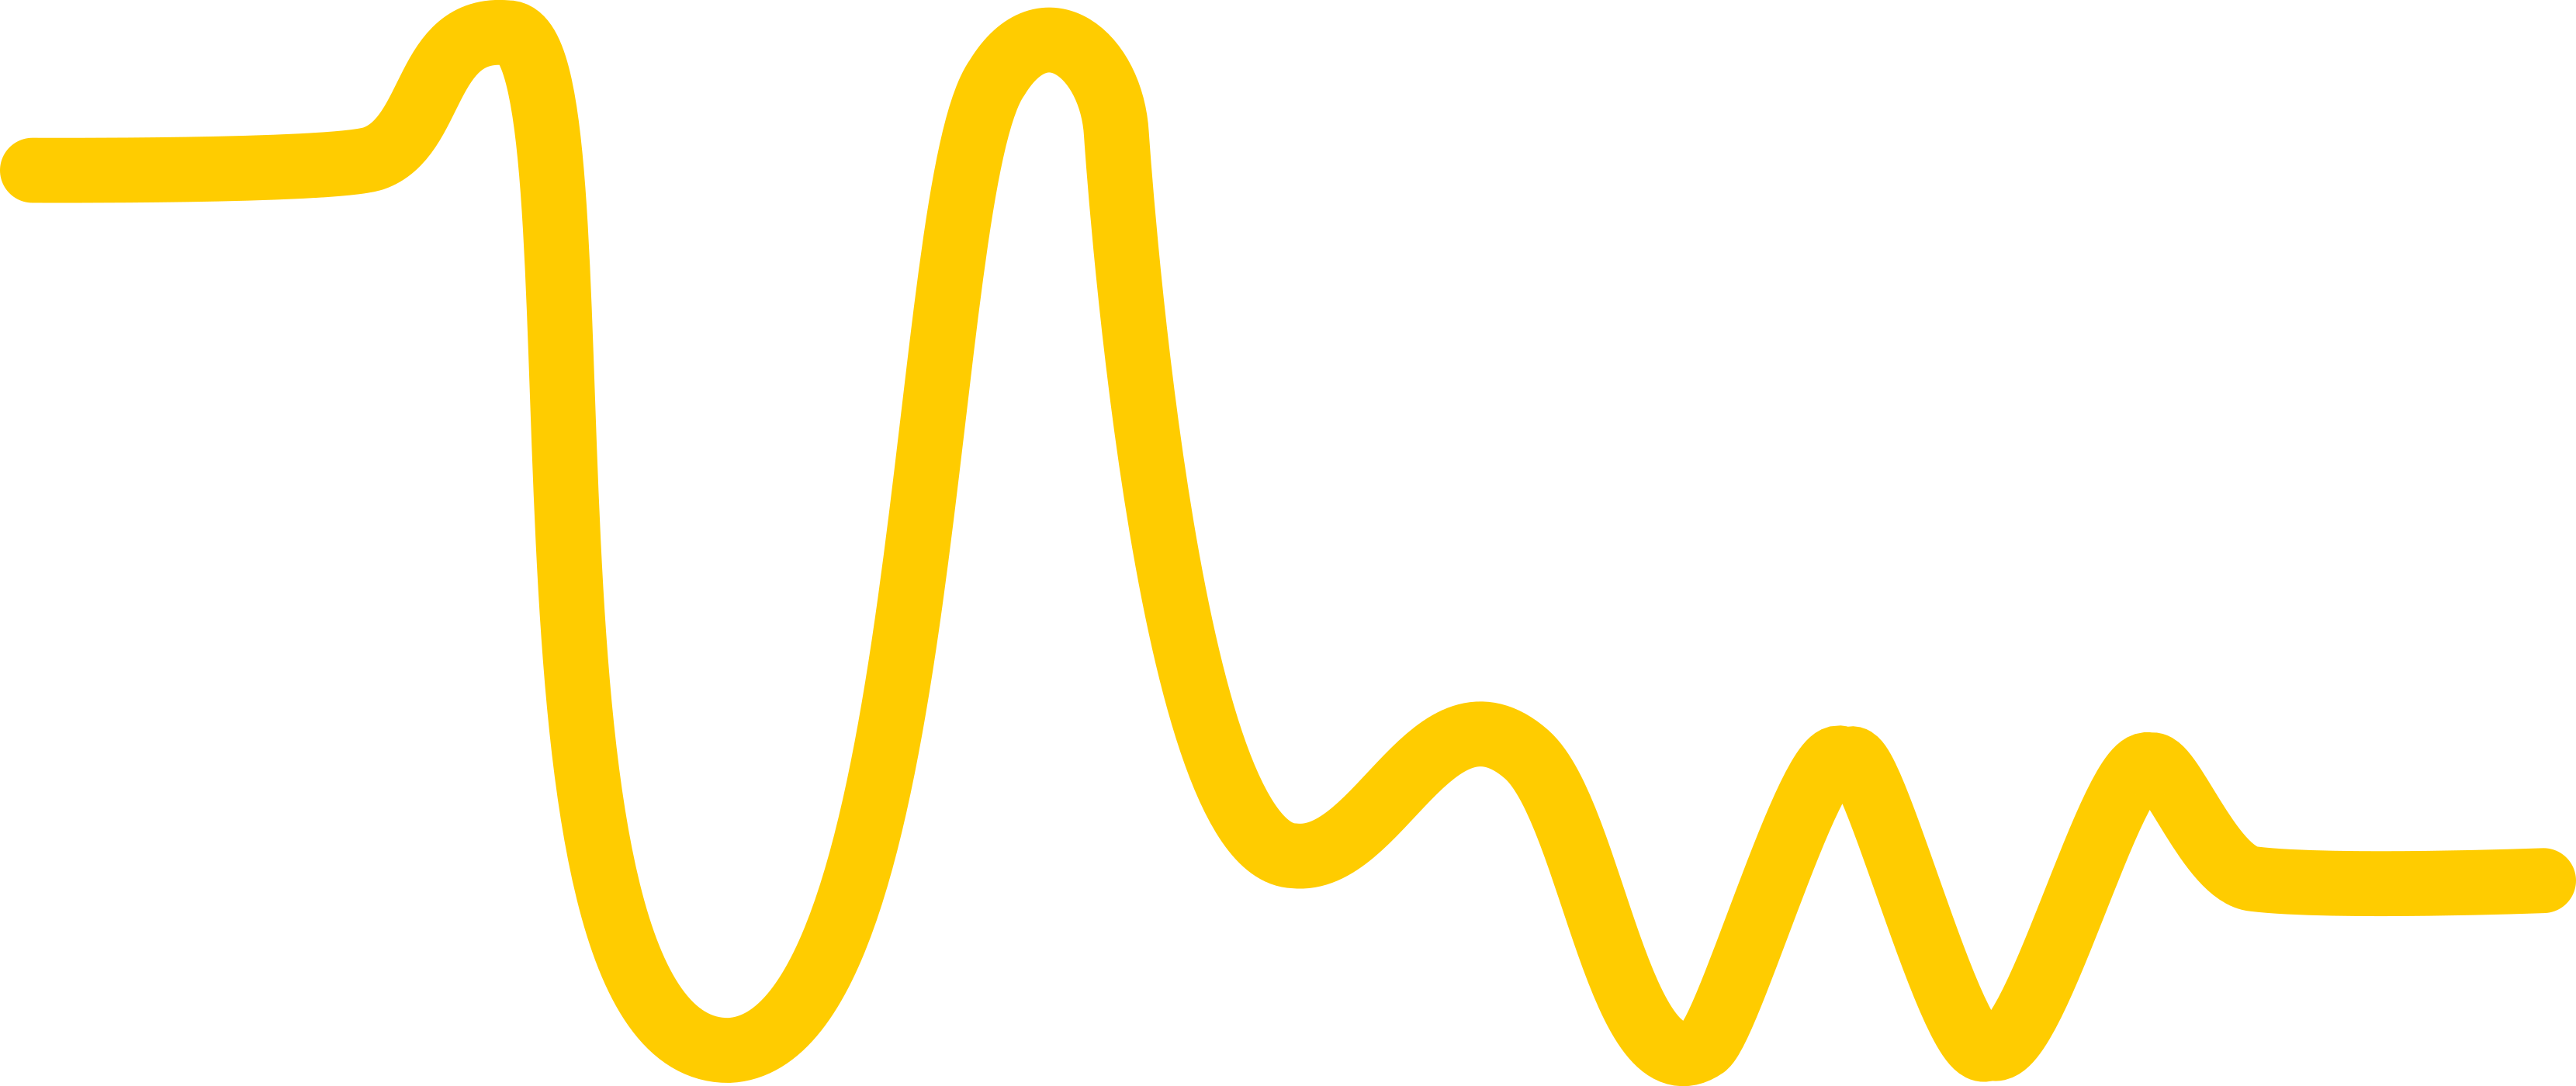
\includegraphics[width=0.3\linewidth]{logo_visuwalk.png} 
\end{center}VISUWALK} %Titre du fichier .pdf
% \cours{Nom du cours} %Nom du cours
% \sujet{Sujet du rapport} %Nom du sujet


%----------- Initialisation -------------------
        
\fairemarges %Afficher les marges
\fairepagedegarde %Créer la page de garde
\tableofcontents%Créer la table de matières
\newpage

%------------ Corps du rapport ----------------
\section{Abstract}


For this semester project, to aid the 2.2 billion visually impaired persons in the world, we were asked to develop a system capable of guiding the latter following a line.\\ Despite the access to multiple technologies capable of helping them navigate, they are for the most part not fit for sports. The most popular solution being the white cane : it is very efficient but not so practical, as it needs a lot of practice to use it and prevents you from using both of your arms/hands if you want to do something.\\For this purpose, we developed Visuwalk for this semester project, a device able to guide you in following a line through audio feedback.\\
The tools we were given for project are a Raspberry Pi and its camera. The main goals of this project are the following :\\
- Detecting the line from the Raspberry Pi’s camera\\
- Process the information given by the line\\
- Generate sound cues to guide the user

\section {User manual}

In order to use our software on your own device, just flash the Visuwalk flavoured Raspbian image from our \href{https://gitlab.eurecom.fr/algh2/visuwalk/-/releases}{Gitlab page}, onto your SD Card. However, if you have got some issues, or an existing installation that you don't want to mess up, make sure you have the \verb|python3-numpy|, \verb|python3-pyaudio|, \verb|python3-opencv| and \verb|python3-picamera| installed on your device, copy the Python scripts that are in the \verb|rasp_prod/| folder of our repository, and execute \verb|main.py|.

\section{Technical manual}

\subsection{Introduction to the Raspberry Pi and Matlab/Simulink
}
    
The first steps towards this project were to connect the Raspberry Pi to our computers and to discover Matlab, which were not easy tasks.
The whole installation was quite lengthy, and did not work for most of us. And if it did work, we then had to connect the camera to the Raspberry Pi, which was also quite hard. So hard that we even thought our camera was broken, until we tested it on other computers, which took a lot of time. In the end, we were left with only 2 Raspberry Pi connected and 2 cameras (Alexandre bought one himself).\\
Concerning Matlab and Simulink, some of us had already used these softwares, but only on surface-level, so we pretty much had to learn from scratch how to use them and more specifically, how to use them with the Raspberry Pi. And this last part was complicated, leading us to this next paragraph.

\subsection{Choosing between Python and Matlab/Simulink
}

The option of using Python showed up because other groups had issues just like us and switched to Python. Thus, we talked about the switch, and decided not to switch completely as we had already advanced on the Matlab code. Instead, we let Guillaume,in parallel, try to do the video processing part (that was done on Matlab) on Python, to see how easier (or harder) it would be.\\
It was much easier and produced better results.And so we were left with one last question : should we also do the sound generation part on Python ?
We were quite reluctant at first, given that almost the whole code was already done in Simulink and that switching and translating it all would take an important amount of time. Besides, we searched and found multiple ways to make a bridge between Python and Simulink. But time was ticking and we still had not found a way to make any of these bridges work correctly, so we made the switch. And it did not take as long as we expected, despite the issues we encountered. \\
Still, we found some interesting features like the C code generation in Matlab/Simulink, which would be used to embed the program on a portable system. Knowing that shared memory in C is possible and probably easier than in Matlab, we searched for a way to use shared memory in Python, and to manually modify the C generated code to implement the share of memory between the sound generation part and the Python video processing, so that the second could indicate the direction to the first.\\
\subsection{Image processing}
\vspace{3mm}
\begin{flushleft}
    \textbf{\large{First discarded idea}}
\end{flushleft}
The first idea we had was to horizontally cut the frame in 2 and process each of them.\\On the upper frame, we would calculate the angle between the middle of the frame and the detected line. On the bottom frame, we would calculate the distance between the detected line and the middle of the frame and this distance would tell us whether the user was standing on the right, left or directly on the line.\\ However, we discarded this idea as the calculation of both the angle and distance were not accurate and neither was the instruction. Indeed, rather than taking the fastest path, it would force the user to always stay on the line, leading to weird routes and sharp turns.
So we changed our approach to the one explained in the following paragraph.
\begin{flushleft}
    \textbf{\large{Final approach for the image processing part}}
\end{flushleft}
The first step toward computing the image and giving an angle is the image acquisition. We use the python library \verb|picamera| in order to get the camera's images, at a quite low quality, because it has proven to be more time-efficient.\\
\begin{center}
\begin{tikzpicture}[scale=3]
\draw[-latex] (0,0) -- (1,0);
\draw[-latex] (0,0) -- (0,-1);
\draw (0.1,-0.1) rectangle (0.9, -0.9);
\draw (0.5,-0.5) node {image};
\draw (1,0) node[right] {\(x\)};
\draw (0,-1) node[below] {\(y\)};
\end{tikzpicture}
\captionof{figure}{OpenCV x and y axis representation}
\end{center}
The frames are then read by openCV and converted into grey. OpenCV represents images with matrices whose indexes may also be seen as coordinate of the following base. An image pixel is then characterized by its coordinate in the following order: \verb|image[y,x]| (matrix line, matrix column).\\We then apply a bilateral filter to the image, as it is a filter that preserve the sharp edges and smooth the rest of the image: this is exactly what we need, especially as there is a pattern with lines on the carpet of the Marconi amphiteater that needs to be removed and finally, we apply a canny edge detector, giving us the following image:\\
\begin{center}
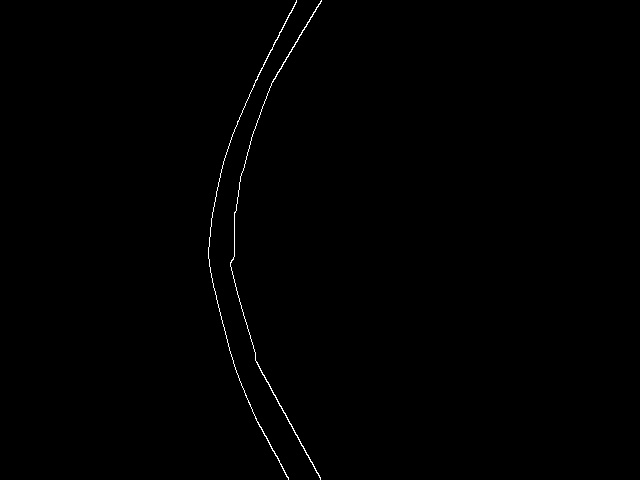
\includegraphics[width=0.35\linewidth]{canny_edge.jpg}
\captionof{figure}{Fully filtered image of the line}
\end{center}
After having a clear image of the line, we apply the Hough transform which will give us a set of straight lines detected on the image. But before calculating any angle, we need to reorient the lines accordingly to our purpose. Indeed, openCV will return us vectors that are oriented towards increasing \(x\), but we need to have them all in the same directon as \(y\), because the user moves on the y axis.

% place le ou tu veux comme tu veux Gui
\begin{center}
    \begin{tikzpicture}[scale=2]
  \draw[-latex] (0,0) -- (0,-1);
  \draw (0,-1) node[below] {\(y\)};

  \draw (0.7,-0.3) -- (1.2,-1.1);
  \draw (1.2,-1.5) -- (0.7,-2.3);

  \draw[->] (1.4, -0.6) -- (1.6, -0.6);
  \draw[->] (1.4, -1.9) -- (1.6, -1.9);

  \draw[->] (2,-0.3) -- (2.5,-1.1);
  \draw[<-] (2.5,-1.5) -- (2,-2.3);

  \draw[->] (2.7, -1.9) -- (2.9, -1.9);

  \draw[->] (3.7,-1.5) -- (3.2,-2.3);
\end{tikzpicture}
\captionof{figure}{popo}
\end{center}
Afterwards, we consider only the bottom of the frame and we compute the \textit{oriented} angle of each vector \(v_i\) with the \(y\) axis (defined as the \(\alpha\) angle), using:
\[ {\alpha}_i = \text{sign}(x) \text{arcos}\left(\frac{y_i}{\|v_i\|}\right) \]
This angle is effectively the one that has our interest, since it is the same if we flip the vectors in the other direction along the \(y\) axis.
Then we calculate the average of the \(\alpha_i\) angles, which gives us our final \(\alpha\).\\
In the case the user is not on the line, we had the following strategy to get him back to it: we calculate the angle between the user and a target zone of the line where we want the person to go. As the evaluation is a race, and as a failure could not worsen anything by itself (we count the number of failures and not their durations), we put the target zone a little bit ahead of the line, so that the user gets back to it quickly. This angle has been called the \(\beta\) angle.\\
\begin{center}
    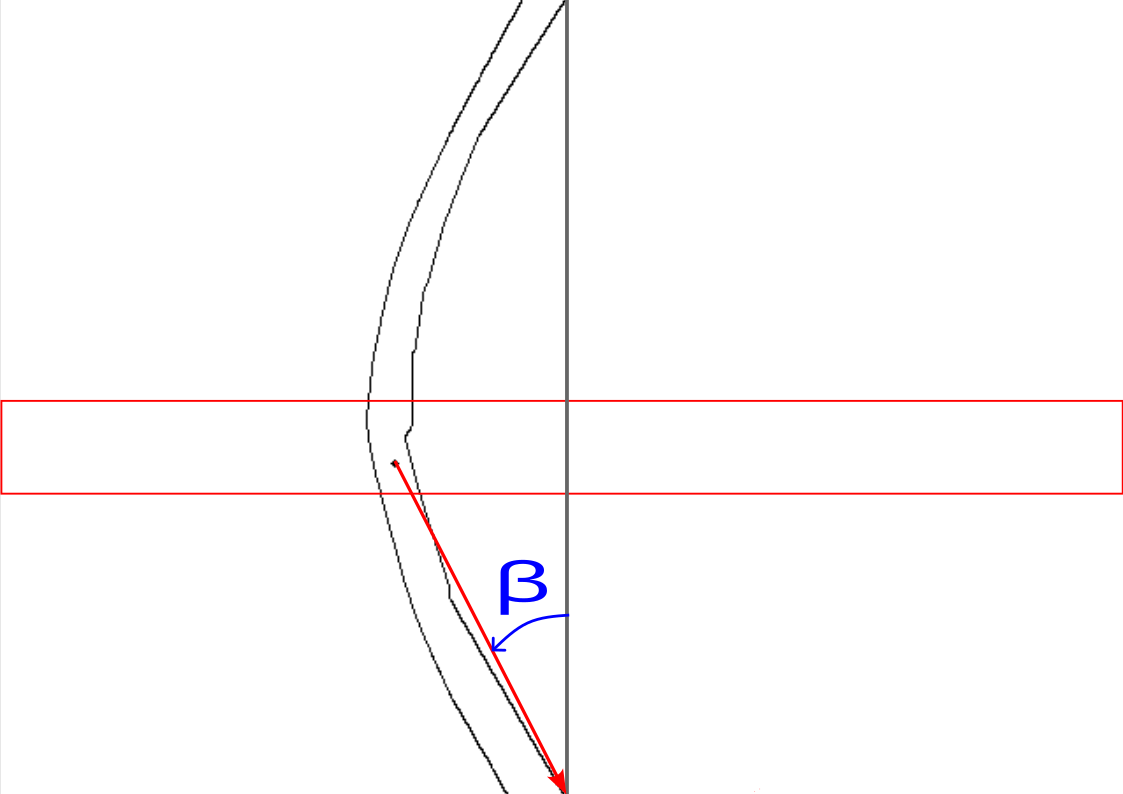
\includegraphics[width=0.3\linewidth]{angle_beta_barycentre_targetpoint.png}
    \captionof{figure}{Representation of the \(\beta\) angle}
\end{center}
In order to compute it, we take a portion of the image vertically, and look at the barycentre of the pixels that were detected as an edge. Then we have a vector between the barycentre and the user (bottom middle horizontally), which angle with the \(y\) axis is computed the same way as for the \(\alpha_i\).\\We have to know when to take the \(\beta\) angle into account. For this, we compute the distance between the user and the bottom of the line, parameter we call \(d\). The method is the same as for the target zone: we compute the barycentre of a portion of the pixels that were detected as edges, and then we just count the distance in pixels between the middle of the image and this barycentre (only along the \(x\) axis).\\
\begin{center}
    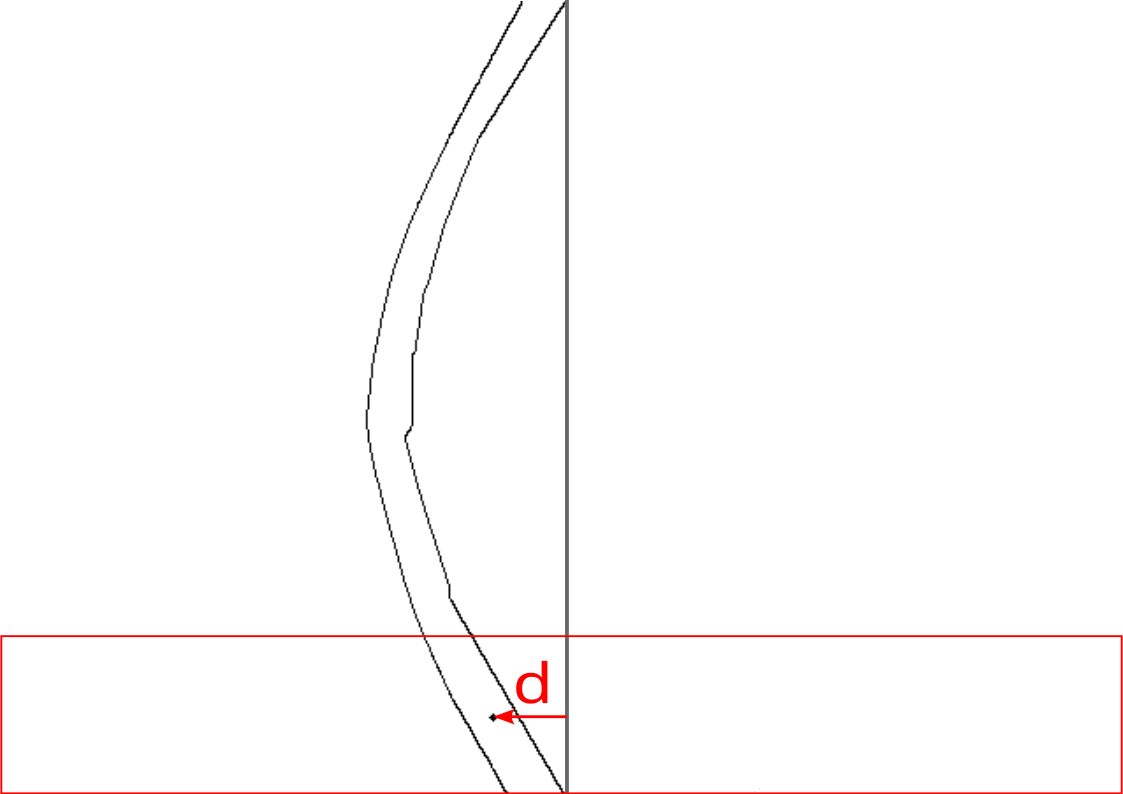
\includegraphics[width=0.3\linewidth]{distance_bas_barycentre.png}
    \captionof{figure}{Representation of the distance \(d\)}
\end{center}
If there is no line in the portion where we look for it, we then only take the \(beta\) angle into account, because that means that the user is very far from the line and should first get back to it. Otherwise, we mix the \(\alpha\) and the \(\beta\) angle relatively to the \(d\) parameter, so that the further the user is from the line, the more we take the second angle into account.\\

We use a \(d\)-dependant weight function, which is

\[ f(d) = (1 - e^{\frac{-d}{\tau}}) \]

We choose \(\tau\) so that when we are at the image extremity, the value of \(f\) is \(0.95\). Thus we have
\[ 3\tau = \frac{\text{width}}{2}, \quad \tau = \frac{\text{width}}{6} \]
It follows,
\[f(d) = 1 - e^{\frac{-6d}{w}}\]

Then, for the angle communicated to the user, called \(\gamma\), we choose this expression to have the behaviour we explained sooner.

\[ \gamma = (1 - f(d))\alpha + f(d)\beta \]

Hence we have,

\[ \gamma = \alpha + (1 - e^{\frac{-6d}{w}})(\beta - \alpha) \]\\
Before sending \(\gamma\) to the sound generation module, we bound the value of the angle in \([-70°, 70°]\). We also reserve \(\gamma = 100\) when no line is detected on the image. Then we send the angle.\\
\textit{Note:} would we have a cover to fix the raspberry on the body, could we better tune the position of the zones we look at, because we know the Raspberry's camera aperture, and giving the average height of a body, we know which distance we cover with camera and what pixel corresponds to what position in real life.

\subsection{Description of source files directory}

In the folder of the source code archive, you will find the \verb|rasp_prod| folder, containing the production source code for the raspberry device, the \verb|improc| and \verb|soundproc| folder containing our test codes for development, and the case folder containing some aborted concept protection and fixation covers for the raspberry.

\subsection{Packaging}

We used pi-gen to generated a Visuwalk flavoured Raspbian image, installing the needed packages and the source files, and running the software at startup. See \href{https://github.com/RPi-Distro/pi-gen}{this}.

\section{Conclusion}

We achieved the main goal of this project : guiding a visually impaired person to follow a line. However, with more time on our hands, we could drastically improve this project.\\
Firstly, the handling of the device. We wanted to 3D print a PLA casing to put the device in, so that the user could wear it on his belt and move freely, without having to hold the Raspberry Pi. Not only would it be more practical, it would also improve the performance of the system by fixing the camera orientation and angle relative to the ground, allowing us to fine tune parameters in the code.\\
\begin{center}
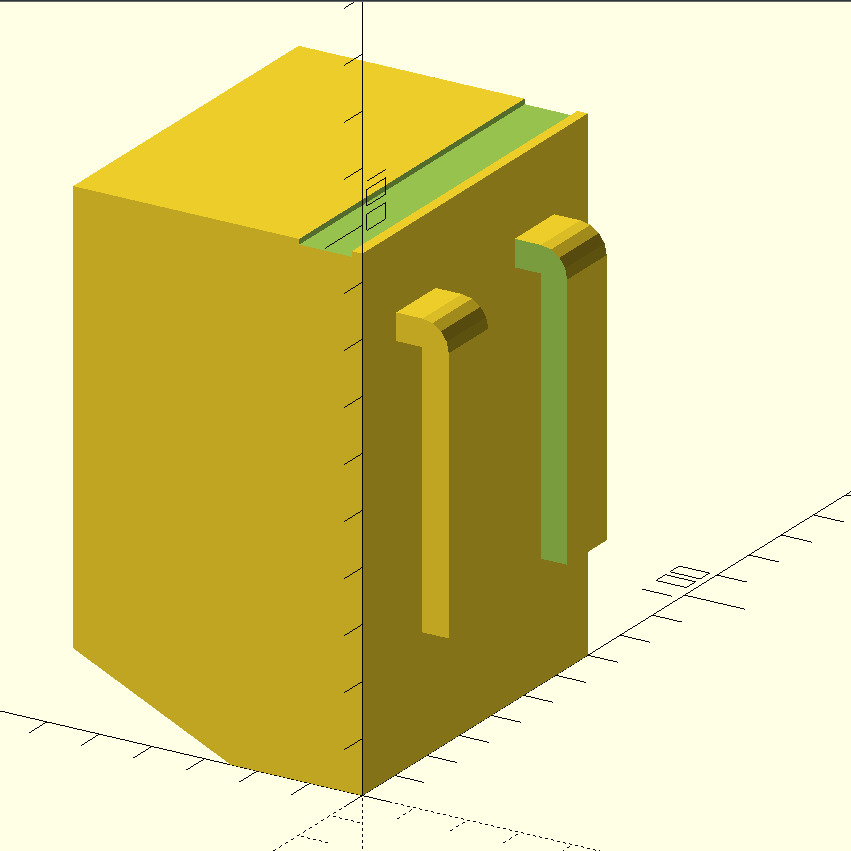
\includegraphics[width=0.2\linewidth]{visuwalk_case1.png}
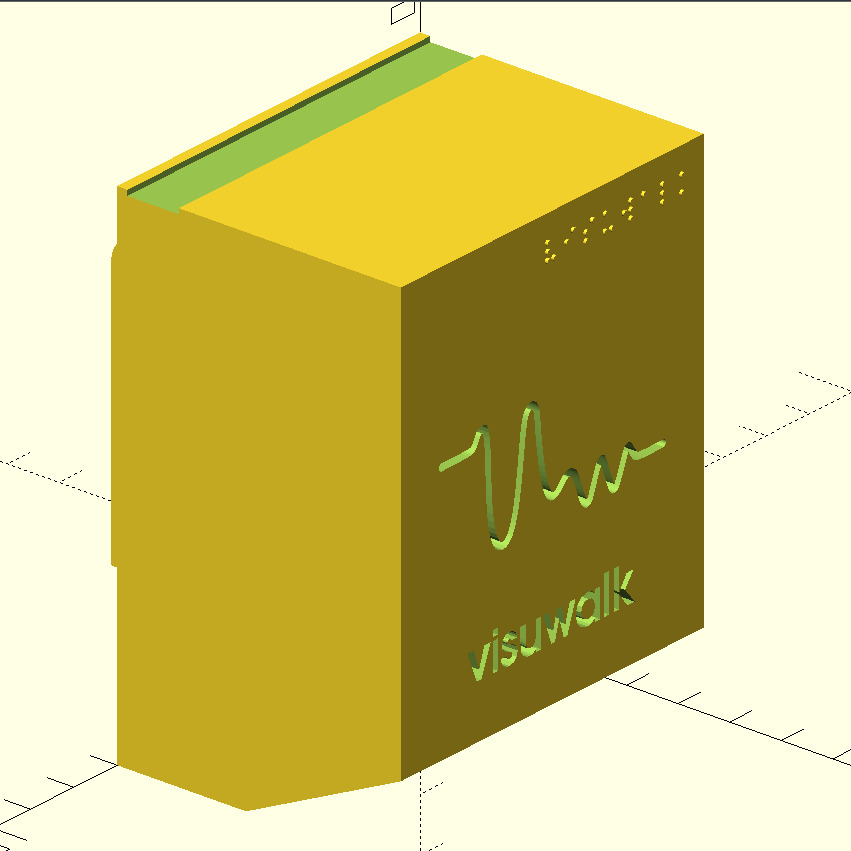
\includegraphics[width=0.2\linewidth]{visuwalk_case2.png}
\captionof{figure}{3D models for possible casing of the device}
\end{center}
Another major improvement is the sound of the instruction. As of now, it is functional, but not really nice to the ears. The objective would be to have a sound that is not too invasive and loud, but also gives accurate instructions.\\
And to give even more accurate instructions, we would also have to reduce the latency between the moment the frame is captured and the moment the sound is in the user's ears. To do so, we intended on launching the image processing part and the sound generation part asynchronously. This way, the two processes would communicate without having to wait for one another.\\
Regarding the business strategy, we thought about putting our source code in open source, allowing everyone to copy it, tweak it and upgrade it to their needs. The benefits we would make from Visuwalk (if we were to be a company) would come from us providing technical support and repair services for the device, lenghtening its lifetime.Thus Visuwalk would be a project fitting in a circular economy dynamic.



\end{document}
